\documentclass[12pt]{scrbook}
\usepackage[utf8]{inputenc}
\usepackage{algorithm}
\setlength{\textfloatsep}{10pt} % Reduces space after the pseudocode
\usepackage{algorithmic}

\usepackage{amsmath}
\usepackage{amssymb}
\usepackage[backend=biber,style=numeric,]{biblatex}
\usepackage{bookmark}
\usepackage{booktabs}
\usepackage{calc}
\usepackage{color}
\usepackage{enumitem}
\usepackage{float}
\usepackage[top=3.0cm, bottom=3.0cm]{geometry}
\usepackage{graphicx}
\usepackage{hyperref}
\usepackage{listings}
\usepackage{MnSymbol}
\usepackage{pgfplots}
\usepackage{pdfpages}
\usepackage{rotating}
\usepackage{scrhack}
\usepackage[automark,ilines]{scrlayer-scrpage}
\usepackage{setspace}
\usepackage{soul}
\usepackage{tabularx}
\usepackage{tikz}

\usepackage{etoolbox}
% decrease the space between headlines and text
\makeatletter
\renewcommand{\chapterheadstartvskip}{\vspace{0pt}}
\renewcommand{\chapterheadendvskip}{\vspace{\baselineskip}}
% \patchcmd{<cmd>}{<search>}{<replace>}{<success>}{<failure>}
\patchcmd{\section}{-3.5ex \@plus -1ex \@minus -.2ex}{-\z@}{}{}
\patchcmd{\section}{2.3ex \@plus .2ex}{-
1ex}{}{}
\patchcmd{\subsection}{-3.25ex\@plus -1ex \@minus -.2ex}{-\z@}{}{}
\patchcmd{\subsection}{1.5ex \@plus .2ex}{-1ex}{}{}
\patchcmd{\@xsect}{\ignorespaces}{\vspace*{0.1\baselineskip}\ignorespaces}{}{}
\makeatother

\usetikzlibrary{positioning, quotes, calc, patterns}
\pgfplotsset{compat=newest}

% Set the page style and center the page number
\pagestyle{scrplain}
\cfoot[\pagemark]{\pagemark} % Center the page number in the footer
\ofoot[]{} % Clear the default outer footer
\ifoot[]{} % Clear the default inner footer

\graphicspath{ {images/} }
\addbibresource{literature.bib}

\definecolor{gray}{rgb}{0.5,0.5,0.5}
\definecolor{darkgreen}{rgb}{0.055, 0.549, 0.153}
\definecolor{midgreen}{rgb}{0, 0.549, 0.082}
\definecolor{mauve}{rgb}{0.58,0,0.82}
\definecolor{blind-purple}{rgb}{0.863, 0.149, 0.498}
\definecolor{blind-blue}{rgb}{0.118, 0.067, 0.773}
\definecolor{blind-orange}{rgb}{0.996, 0.38, 0}
\definecolor{blind-turquoise}{rgb}{0, 0.584, 0.62}
%
\lstset{frame=tb,
    language=SQL,
    aboveskip=3mm,
    belowskip=3mm,
    showstringspaces=false,
    columns=flexible,
    basicstyle={\small\ttfamily},
    numbers=none,
    numberstyle=\tiny\color{gray},
    keywordstyle=\color{blue},
    commentstyle=\color{darkgreen},
    stringstyle=\color{mauve},
    breaklines=true,
    breakatwhitespace=true,
    tabsize=3 
}
%\raggedbottom
\renewcommand{\arraystretch}{1.3}  % Increase row height for better readability

\begin{document}

\newgeometry{top=3.0cm, bottom=3.0cm, left=4cm, right=2cm}
\begin{titlepage}
    \begin{center}

        \begin{spacing}{1.5}
            
\includegraphics[scale=0.25]{images/Bildmarke_blue_8cm.jpg}
            \vspace*{\fill}
        \end{spacing}
        \begin{spacing}{2.5}
            \textbf{\huge Efficient Implementation and Evaluation of Einstein Summation via Batched Matrix Multiplication}\\[0.5cm]
            \vspace*{\fill}
            \begin{spacing}{1.5}
                \textbf{PROJECT WORK\\}
                Autumn Semester 2024/2025
            \end{spacing}
        \end{spacing}

        \vspace*{\fill}

        \begin{spacing}{1.15}
            \textbf{FRIEDRICH-SCHILLER-UNIVERSITY JENA\\}
            Faculty for Mathematics and Computer Science

            \vspace*{\fill}

            \textit{Submitted by Fenja Wagner}\\
            Student ID Number: 177944\\
            Supervisor: Mark Blacher\\
            Jena, \today

        \end{spacing}
    \end{center}
\end{titlepage}

\chapter*{Abstract}
Tensor contractions are a fundamental operation in many scientific computing and machine learning applications, but their complexity and large memory demands often make them a performance bottleneck.
Different approaches to computing tensor contractions come with different trade-offs — depending on the design of the algorithm, certain methods are better suited for small or simple pairwise contractions, while others can handle only complex tensor expressions more efficiently.
Additionaly, many existing implementations are restricted to specific data types and tensor expressions or  can only process a small number of tensors, limiting the execution of multi-tensor contractions versatility.\\
In this project, we present a relatively simple custom implementation for computing tensor contractions, based on the Tensor-Transpose-Batch-GEMM-Transpose (TTBT) approach and expressed using the concise and powerful modern Einstein summation notation. Despite its simplicity, our algorithm is capable of handling arbitrarily large and complex tensor expressions.\\
The comparison of our implementation against two widely used libraries, Numpy~\cite{Numpy} and PyTorch~\cite{PyTorch}, both of which support Einstein summation, shows that our implementation can compete with both libraries, outperforming NumPy in compute-intensive scenarios. These findings show that it is possible to build a custom tensor contraction engine that stays flexible and efficient, handling complex tensor expressions while still keeping up with well-established libraries.

%
\chapter*{Zusammenfassung}
Tensorkontraktionen spielen eine zentrale Rolle in vielen wissenschaftlichen Berechnungen und Anwendungen des maschinellen Lernens. Allerdings sind Tensoroperationen oft speicherintensiv und rechenaufwändig und werden dadurch schnell zu einem Bottleneck in Berechnungen. 
Unterschiedliche Lösungsansätze bringen dabei unterschiedliche Vor- und Nachteile mit sich: Während einige Methoden besonders gut für die Berechnung paarweiser Kontraktionen oder kleiner Tensornetzwerkkontraktionen geeignet sind, sind andere wiederum performant auf großen Tensorkontraktionen.
Viele bisherige Implementierungen sind zudem auf bestimmte Datentypen und Tensorstrukturen beschränkt oder können nur eine begrenzte Anzahl von Tensoren verarbeiten, wodurch die Berechnung von Ausdrücken mit vielen Tensoren problematisch wird.\\

\noindent In diesem Projekt stellen wir eine relativ einfache Implementierung zur Berechnung von Tensor-Kontraktionen vor, die auch große und komplexe Tensorkontraktionen effizient berechnen kann. Sie basiert auf dem Transpose-Transpose-BMM-Transpose-Ansatz (TTBT) und nutzt die moderne Einsteinsche Summenkonvention zur Formulierung der zu berechnenden Kontraktion.
Ein Vergleich mit den weit verbreiteten Bibliotheken NumPy~\cite{Numpy} und PyTorch~\cite{PyTorch}, die ebenfalls die Einsteinsche Summenkonvention unterstützen, zeigt, dass unser Ansatz nicht nur konkurrenzfähig ist, sondern in rechenintensiven Szenarien sogar deutlich besser als NumPy abschneidet. Unsere Ergebnisse belegen, dass es möglich ist, eine eigene Tensor-Kontraktions-Engine zu entwickeln, die flexibel, effizient und leistungsstark ist und dabei mit etablierten Bibliotheken mithalten kann.
%
\tableofcontents
%
\newgeometry{top=3.0cm, bottom=3.0cm, left=4cm, right=2cm}
%
\chapter{Introduction}
\label{introduction}
Tensor contractions play an important role in many scientific and machine learning applications. However, due to their complexity and large memory requirements, they can quickly become a performance bottleneck. 
As a result, developing efficient solutions for this class of problems is of great interest. \\
Although various approaches to computing tensor contractions exist, each comes with its own limitations. While some implementations are efficient only for small tensors and perform poorly for compute-bound problems, others are restricted to simple tensor networks structures or specific data types. In this project, our goal is to implement a promising approach to tensor contractions that can handle a wide range of tensor structures and data types, and to compare it to existing engines.\\

\noindent Tensor contractions can be expressed elegantly using the so-called modern Einstein summation notation. The original notation was introduced by Albert Einstein in 1916, from which its modern form is derived ~\cite{einstein}. While brief and concise, it allows for the clear representation of various tensor operations, including element-wise multiplications, dot products, outer products, and matrix multiplications. Since these expressions can be combined, even complex tensor networks can be described in a simple and readable form using Einstein summation. As a result, well-established libraries such as NumPy ~\cite{Numpy} and PyTorch ~\cite{PyTorch} have integrated this notation into their tensor contraction engines. In this project, we adopt the Einstein summation convention to compute tensor contractions. Our goal is to support the contractions that can be expressed with this convention, allowing us to handle complicated tensor structures.\\

\noindent We then compare our implementation to two different established libraries Numpy ~\cite{Numpy} and PyTorch ~\cite{PyTorch}, both of which included Einstein summation into their tensor contraction engines. PyTorch broadly follows the same approach as our implementation, mapping the tensor contraction to a batch matrix multiplication, but relies among others on highly optimized libraries for linear algebra operations for that operation. Numpy uses a different strategy and iterates over the indices of the problem. We find that our implementation is able to compete with both of these engines, being more efficient than Numpy for compute-intensive problems.
 The code to our implementation can be found on \url{https://github.com/fenjaWagner/TTBMMT}.\\
 
 \noindent This paper is structured as follows: We first provide the necessary background information in Section \ref{background} and explain tensors, Einstein summation notation and tensor contractions. In Section \ref{related} we explore different approaches to tensor contractions as well as contraction paths and existing implementations. Then we will describe our algorithm in detail in Section \ref{algorithm}, presenting the benchmark results in Section \ref{experiments}. Finally, we will discuss these results in Section \ref{discussion} and point out possible improvements to our solution.

%
\chapter{Background}
\label{background}
\section{Tensors}
Tensors are algebraic objects that extend the concept of scalars, vectors, and matrices to higher dimensions and can be interpreted as a multi-dimensional array. The number of dimensions is usually called the ``rank'' or ``order'' of a tensor. A scalar, for example, can represent a zero-order tensor, a vector a first-order tensor, and a matrix a second-order tensor. Higher-order tensors have multiple dimensions. 
Each of these dimensions of a tensor is represented by an index. 
A tensor of order $ n $ can be written as $ T_{i_1 i_2 \dots i_n} $, where each index $ i_k $ runs over a certain range.
The size of a tensor is determined by the product of the values of each index’s range.

\section{Tensor Contractions}
\noindent Tensor contraction is an operation that reduces the order of one or more tensors by summing over their shared indices. It generalizes the concept of matrix multiplication, where summation occurs over a shared index. \\
For example, for matrices $A\in \mathbb{R}^{m\times p}$ and $B\in \mathbb{R}^{p\times n}$ , the result is a new matrix $C\in \mathbb{R}^{m\times n}$, computed as:
$$
C_{ij} = \sum_{k} A_{ik} B_{kj}
$$

\noindent For higher order tensors, the idea can be extended as follows: Let $T\in \mathbb{R}^{i_1\times ... \times i_p\times k_1 \times ... \times k_r}$ and $S\in \mathbb{R}^{k_1 \times ... \times k_r\times j_1 \times ... \times j_q}$. Then,

$$
C_{i_1, \dots, i_p, j_1, \dots, j_q} = \sum_{k_1, \dots, k_r} T_{i_1, \dots, i_p, k_1, \dots, k_r} S_{k_1, \dots, k_r, j_1, \dots, j_q}
$$

\noindent where the indices $ k_1, \dots, k_r $ are summed over, reducing the total number of dimensions in the resulting tensor $ C $.

\section{Tensor Networks}
A tensor network represents a complex tensor expression as a graph. Each tensor is represented by a node, and the indices of the tensors are represented by edges. If two tensors share an index, that index is contracted, and an edge connects the two nodes. Tensor networks where more than two tensors share the same index are called ``hypernetworks''. 

\begin{figure}
\begin{center}
\begin{tikzpicture}
    % Nodes (Tensors)
    \node[circle, draw, minimum size=1cm] (A) at (1, 0) {$A$};
    \node[circle, draw, minimum size=1cm] (B) at (3, 0) {$B$};

    % Edges (Contractions)
    \draw[-] (A) -- (B) node[midway, below] {$i$};

    % External Legs (Free indices)
    \draw[-] (A) -- (0, 1) node[left] {$j$};
    \draw[-] (A) -- (0, -1) node[left] {$k$};
    \draw[-] (B) -- (4, 1) node[right] {$l$};
    \draw[-] (B) -- (4, -1) node[right] {$m$};
\end{tikzpicture}
\caption{A three-dimensional tensor $T_{p,q,r}$ and a tensor network of two tensors $A$, $B$ with shared index $i$.}
\label{fig:tensor_network}
\end{center}
\end{figure}

\noindent In Figure \ref{fig:tensor_network} one can see a tensor network representing the tensor contraction 
$$
C_{jklm} = \sum_{i} A_{jki} B_{ilm}.
$$

\section{Einstein Summation}
The modern Einstein summation convention is a notation used in tensor calculus that simplifies mathematical expressions. The original convention consists of eliminating the need to explicitly write summation signs by implicitly contracting all indices that are repeated in the input term. \\
In the example above, the tensor contraction would be represented as
$$C_{jklm} = A_{jki} B_{ilm} ,$$
\noindent where the index $i$ is summed over because it appears in the index sets of both $A$ and $B$.\\
This idea is extended in the modern Einstein summation convention by contracting all indices that do not appear in the output term. In modern Einstein summation, our example can be written as
$$A_{jki} B_{ilm} \rightarrow C_{jklm}.$$

This extension leads to an even more powerful formalism. By stating explicitly the indices and their order in the output tensor, we can also express other tensor operations as transpositions, dot products, traces, and outer products in this concise manner.
For example, the expression
$$A_{jki} B_{ilm} \rightarrow C_{klj}$$
means contracting the tensors via the index $i$, taking the result and summing over the axis $m$ (since the index $m$ does not appear in the output tensor) and transposing the tensor to $ C_{klj}$. \\

\noindent When using common Einstein summation APIs such as Numpy ~\cite{Numpy} or PyTorch ~\cite{PyTorch}, the equation is expressed by stating simply the input and output indices as a format string. The format string for our last example would be
$$jki, ilm \rightarrow klj.$$

\noindent In the following, we will refer to the Einstein summation convention as ``einsum'' and use the representation as a format string with the output tensor explicitly marked by an arrow.


\chapter{Related Work}
\label{related}
\section{Calculating Tensor Contractions}
\textcite{springer} state that even though the concept of tensor contractions is quite similar to matrix multiplications, the calculation of these contractions is usually inefficient compared to highly optimized algorithms for matrix multiplications. However, when performing tensor contractions, there are several methods to improve the performance, depending on the characteristics of the tensor and the hardware architecture. \textcite{springer} describe three different approaches to calculating tensor contractions that are used by known tensor contraction libraries.  

\subsection{Nested Loops}
The first and most straightforward approach mentioned by Springer and Bientinesi~\cite{springer} involves nested loops, where the indices of the tensors are iterated over. Each loop corresponds to an index of the tensor, and the contraction is achieved by summing over the repeated indices. However, this approach can suffer from poor memory access patterns, especially when the tensors are complex and large, which often leads to suboptimal memory access patterns. Some of these inefficiencies can be mitigated by applying vectorization, loop transformations such as loop reordering or loop fusion that optimize cache efficiency.\\
Numpy~\cite{Numpy} implements their einsum summation in loops by lowering the expression into a very general form and using a Numpy native iterator loop that effectively becomes a loop-based kernel.

\subsection{Loops-over-GEMMs}
The Loops-over-GEMMs method slices a tensor into multiple 2D sub-tensors (matrices) and contracts them using General Matrix Multiplication (GEMM) operations. This approach is particularly effective when the sub-tensors are large, as it allows efficient use of optimized GEMM routines. However, in some cases, the 2D slices may be small or require strided memory access, which can degrade performance~\cite{springer}.

\subsection{Transpose-Transpose-GEMM-Transpose (TTGT)}
Another method that is explained by \textcite{springer} is to transpose and flatten the tensors so that they can be interpreted as matrices. This approach involves transposing and flattening the tensors, multiplying them using a General Matrix Multiply (GEMM) operation, and then transposing the result back to match the output tensor's shape. 
One key insight is that every tensor contraction can be represented as a matrix multiplication by dividing the index sets of the two to-be-contracted tensors $A$ and $B$ and the output tensor $C$ into sets $I_A, I_B$, the indices that appear in both $A$ and $C$ or in $B$ and $C$, and the set $I_{con}$, the contracted indices that appear in both $A$ and $B$ but not in $C$. $A$ is then flattened into a matrix $A' \in \mathbb{R}^{I_A\times I_{con}}$, $B$ into a matrix $B' \in \mathbb{R}^{I_{con} \times I_B}$, the result $A'\times B' = C' \in \mathbb{R}^{I_A\times I_B}$ must then be reshaped and transposed, so its indices match the ones given for $C$.
The advantage of this approach is that it reduces the contraction operation to a matrix multiplication, which is a highly optimized operation in most linear algebra libraries such as BLAS~\cite{BLAS}. However, the need to transpose the tensors and the result introduces an overhead due to additional storage and data movement. The performance of this method is bandwidth-bound if the transposing steps take most of the runtime. In compute-bound scenarios, where the computation is more expensive than the memory transfer, this method can perform very well because GEMM can be highly optimized, especially when using modern hardware, such as GPUs and specialized matrix-multiplication units.

\subsection{GEMM-like Tensor Tensor multiplication (GETT)}\label{gemm}
\noindent \textcite{springer} introduce an approach called ``GEMM-like Tensor Tensor multiplication'' (GETT), that aims to combine the benefits of the aforementioned approaches while avoiding their drawbacks. 
While the concept of GETT is basically similar to that of TTGT, it avoids the overhead of the tensor transposition by implicitly reorganizing the data while packing it into the caches. In the next step, the data that is loaded into the cache can be processed by highly optimized macro-kernels.

\subsection{Transpose-Transpose-BMM-Transpose (TTBT)}
\sloppy
Just as any tensor can be represented as a single matrix, it can also be written in the form of a batched matrix.
By adopting the concept of Transpose–Transpose–GEMM–Transpose, one can replace the GEMM with a batched matrix multiplication (BMM). Similar to the TTGT approach, TTBT usually performs well for compute-bound problems, while the overhead during the pre- and post-processing of the tensors remains a drawback for bandwith-bound calculations.\\
PyTorch’s einsum implementation~\cite{PyTorch} adopts the TTBT approach by partitioning the index set into subsets and mapping the problem to a BMM whenever its structure allows.

\subsection{Code Generation for Specific Problems}
Another approach is to generate optimized code for specific tensor contractions. TACO (the Tensor Algebra Compiler)~\cite{kjolstad2017taco} can generate efficient solutions for both sparse and dense tensor operations. However, since the generated code is tailored to a specific pairwise contraction of two given tensors, TACO lacks the flexibility needed to process arbitrary tensor operations dynamically at runtime.

\section{Contraction Paths}
Since tensor contractions are associative, a multi-tensor contraction can be broken down into a sequence of pairwise tensor contractions. The order of these pairwise contractions, called the ``contraction path'', influences the calculation's performance immensely. Consequently, it is crucial to choose an efficient contraction path, but the computation of these paths is very costly itself. 
Optimized Einsum (opt\_einsum)~\cite{opteinsum} 
is a package for optimizing the tensor contraction order for a problem. For executing pairwise contractions, the user can select from different backends. \textcite{cgreedy} improve the contraction path determination of opt\_einsum and introduce a greedy approach that allows calculating a path either optimized for the size of the biggest intermediate tensor or the total number of floating-point operations needed for the contraction. \textcite{blacher2024einsum} state that choosing the path that optimizes the number of flops does not necessarily result in better performance, since a size-optimized path results in more balanced intermediate tensors and therefore a better cache usage. 

%
\chapter{The Algorithm}
\label{algorithm}
\section{Pairwise Tensor Contraction}

\begin{algorithm}[H]
\caption{\textsc{Custom Pairwise Tensor Contraction}}
    \label{alg:pc}
\begin{algorithmic}[1]
    \REQUIRE $einsum\_string$, Tensors $A$, $B$
        \ENSURE Tensor $C$
        \STATE retreive $I_A , I_B , I_{batch} , I_{contract}$
        \STATE store the sizes of the indices
        \STATE Preprocess $A$: transposing, removing traces and summing over arbitrary axes
        \STATE $A \leftarrow$\textsc{Flatten}($A$)
        \STATE Preprocess $B$: transposing, removing traces and summing over arbitrary axes
        \STATE $B \leftarrow$\textsc{Flatten}($B$) 
        \STATE $C\leftarrow$\textsc{BMM}(A,B)
        \STATE Postprocess $C$: reshape $C\leftarrow C_{i_{{batch}_1}...i_{{batch}_k} i_{{A}_1} ...i_{{A}_l} i_{B_1} ...i_{B_m}}$
        \STATE transpose $C\leftarrow C_{outputIndices}$
        \RETURN $C$
\end{algorithmic}
\end{algorithm}
For our pairwise tensor contraction, we use the TTBT (Transpose Transpose BMM Transpose) approach.
 Given an einsum string $a_1...a_k,b_1...b_l\rightarrow c_1...c_r$ that contains the indices of the input tensors $A_{a_1...a_k},B_{b_1...b_l}$ and the indices of the output tensor $C_{c_1...c_r}$ in the right order, we divide the index sets of the two to-be-contracted tensors $A$ and $B$ and the output tensor $C$ into the four sets
\begin{itemize}
    \item $I_{batch}= \{i_{{batch}_1},...,i_{{batch}_k}\}$, the indices that appear in $A, \text{ }B$ and $C$,
    \item $I_A=\{i_{{A}_1}, ...,i_{{A}_l}\}$, the indices that appear in both $A$ and $C$ but not in $B$,
    \item $I_B= \{i_{B_1} ,...,i_{B_m}\}$, the indices that appear in both $B$ and $C$ but not in $A$,
    \item $I_{contract} = \{ i_{{contract}_1}, ..., i_{{contract}_n}\}$, the contracted indices that appear in both $A$ and $B$ but not in $C$.
\end{itemize}
Consider that all indices appear at most once in the sets, and that indices which appear solely in $A$ or $B$ but not in $C$ are excluded from all four sets. We also store the range of each index in a dictionary.\\
By then transposing $A$
with $indices_A \rightarrow i_{{batch}_1}...i_{{batch}_k}i_{{A}_1} ...i_{{A}_l}i_{{contract}_1} ... i_{{contract}_n}$
to $A'$ and $B$ with $indices_B \rightarrow i_{{batch}_1}...i_{{batch}_k}i_{{contract}_1} ... i_{{contract}_n}i_{{B}_1} ...i_{{B}_m}$ to $B'$. By using Numpy's einsum engine \cite{Numpy}, we not only reorder the indices of the tensors but also eliminate traces and sum over arbitrary axes. This procedure ensures that our implementation can handle all possible einsum expressions. In addition, removing traces and arbitrary indices before the contraction results in smaller tensors and therefore smaller intermediate tensors and a lower number of floating-point operations.\\
 We then calculate the shape of the combined batch dimensions, the combined contracted dimensions, and the combined kept dimensions for $A$ and $B$ by multiplying the ranges of the respective indices.\\
 The result $C'$ is calculated by a blocked and parallelized batched matrix multiplication algorithm that we generated using TACO \cite{kjolstad2017taco} and optimized by blocking to improve cache usage and avoid unnecessary data movement. It is parallelized for problems that exceed a certain size. This algorithm takes the flattened tensors $A$ and $B$ and returns  $C' = A' \times B' \in \mathbb{R}^{\text{size}(I_{batch}) \cdot \text{size}(I_A) \cdot \text{size}(I_B)}$. $C'$ is then reshaped and transposed so its indices and their order match the given output indices. For the pseudocode of our pairwise tensor contraction refer to Algorithm \ref{alg:pc}.  \\
The mapping of the tensors $A$ and $B$ to batched matrices and the remapping of the output tensor $C'$ to the desired shape is processed in Python, while the batched matrix multiplication is written in C++. \\
Our implementation can process int\_16, int\_32, int\_64, float\_32, and float\_64 as data types.


\section{Multi-Tensor Contraction}
\begin{algorithm}[H]
    \caption{\textsc{Multi-Tensor Contraction}}
    \label{alg:mtc}
    \begin{algorithmic}[1]
        \REQUIRE  contraction\_path,  tensor\_list, einsum\_string, backend\_flag 
        \ENSURE Tensor $C$
        \STATE Store the length of tensor\_list in   $t\_l$.
        \STATE Calculate the ssa path from the contraction\_path.
        \STATE Calculate the annotated\_ssa\_path from the ssa path and the einsum\_string. 
        \FOR{every path\_tuple in  annotated\_ssa\_path }
        \STATE Retrieve tensors $A$ and $B$ from tensor\_list with indices from the path\_tuple.
        \STATE  Retrieve the mini\_einsum\_string from the path\_tuple.
        \STATE Set $pc\_method$ depending on the backend\_flag 
        \STATE  $C =$ $pc\_method$($A$, $B$, mini\_einsum\_string, backend\_flag) 
        \IF{index for tensor $A$ $\geq$ $t\_l$ }
        \STATE Delete $ A$ 
        \ENDIF
        \IF{index for tensor $B$ $\geq$ $t\_l$ }
        \STATE Delete $ B$ 
        \ENDIF
        \STATE Append $ C $ to tensor\_list 
        \ENDFOR
        \RETURN  $C$ 
    \end{algorithmic}
\end{algorithm}
Our multi-tensor contraction algorithm takes the einsum string, the list of the referring tensors, a contraction path, and a backend flag. Our algorithm for pairwise contractions can process einsum strings composed of UTF8 symbols. However, PyTorch \cite{PyTorch} and Numpy \cite{Numpy} can only handle alphabetic characters. 
To be able to compare our algorithm to these approaches, we use einsum\_benchmark \cite{blacher2024einsum} to generate an annotated contraction path that contains a list of pairs of indices for the tensors in the tensor list that are to be contracted and the short einsum string for that specific contraction. 
This short einsum string consists only of alphabetic characters. We then perform the pairwise contraction with the backend indicated by the flag. 
We implemented Numpy's and PyTorch's einsum engine and our pairwise contraction as possible backends. Our own implementation will be referred to as ``custom''. Since Numpy's highly optimized matrix multiplication engine can also process batched matrices \cite{Numpy}, we added a fourth backend that consists of our pairwise contraction algorithm in combination with Numpy's matrix multiplication instead of our BMM. We will call this backend ``np\_mm'' to distinguish it from our custom implementation. \\
The result of the pairwise tensor contraction is then appended to the tensor list. If the tensors $A$ or $B$ were not in the original tensor list, they are replaced with a scalar to avoid unnecessary storing of data.\\
For the pseudocode of the multi-tensor contraction refer to Algorithm \ref{alg:mtc}.



%
\chapter{Experiments}
\label{experiments}
We compare our custom tensor contraction algorithm to the einsum engines of PyTorch and Numpy as well as to the np\_mm backend. To evaluate the performance of each engine, we use two different sets of problems: First, we test all four engines on simple pairwise tensor contractions with different structural characteristics. Second, we evaluate the four einsum engines on real-world einsum expressions.\\
\textcite{blacher2024einsum} point out that most current tensor libraries are optimized for a limited range of tensor operations, particularly those involving large, dense tensors. However, real-world applications often require a much broader variety of tensor operations, which can cause performance issues. To solve this problem, they present the einsum\_benchmark dataset that includes a wide range of tensor operations and covers the diverse types of operations used in practice. To address this issue, we assess the performance of all four implementations on 28 real-world problems from that dataset.\\
We measure the iterations per second for all experiments, that is, how often a given einsum expression can be executed within one second. \\
The experiments are performed on a machine with
an Intel i5-7200U 2-core processor running Ubuntu 22.04-1 with 8 GB of RAM.
Each core has a base frequency of 2.5 GHz and a max boost frequency of 3.1 GHz. The evaluation is done in
Python 3.12.8 with PyTorch 2.5.1 and Numpy 2.2.1.

\section{Experiments on Pairwise Tensor Contractions}
We designed four format strings for pairwise tensor contractions with or without batch dimensions, traces and arbitrary indices in different combinations as can be seen in Table \ref{tab:instance:data}.
\begin{table}[H]
    \caption{Format string and properties of the four einsum expressions.}
    \label{tab:instance:data}
    \centering
    { \scriptsize
    \begin{tabularx}{\textwidth}{>
    {\raggedright\arraybackslash}p{3cm} >
    {\centering\arraybackslash}X >
    {\centering\arraybackslash}X >
    {\centering\arraybackslash}X}
        \toprule
        \textbf{Format String} & \textbf{Batch Dimension} & \textbf{Traces} & \textbf{Arbitrary Indices} \\
        \midrule
        $aabcd,adeef\rightarrow dcf$ & yes & yes & yes  \\
        $abcd,adef\rightarrow dbef$ & yes & no & yes  \\
        $aabcd,adeef\rightarrow bcf$ & no  & yes & yes  \\
        $abcd,adef\rightarrow cbef$ & no  & no  & no   \\
        \bottomrule
    \end{tabularx}
    }
\end{table}

\noindent To evaluate the performance of the four einsum engines across scenarios with increasing computational intensity, we repeatedly generated random tensors $A$ and $B$ for each problem, increasing the dimensions for each index in each repetition. For example, the first pair of tensors generated for the einsum expression $aabcd,adeef\rightarrow dcf$ has sizes (2,2,2,2,2) for both tensor $A$ and $B$, resulting in 128 floating point operations (or 2.11 floating point operations if we use a log10 scale), the second one (5,5,5,5,5), and so forth. A table with the dimension sizes and the resulting number of floating point operations for the four problems can be found in Table~\ref{tab:dimensions} in the appendix.\\

\noindent As can be seen in Figure~\ref{flops}, our custom implementation outperformes PyTorch and Numpy for problems that contain batch dimensions, traces and arbitrary indices.
\begin{figure}[h]
    \label{flops}
    \centering
    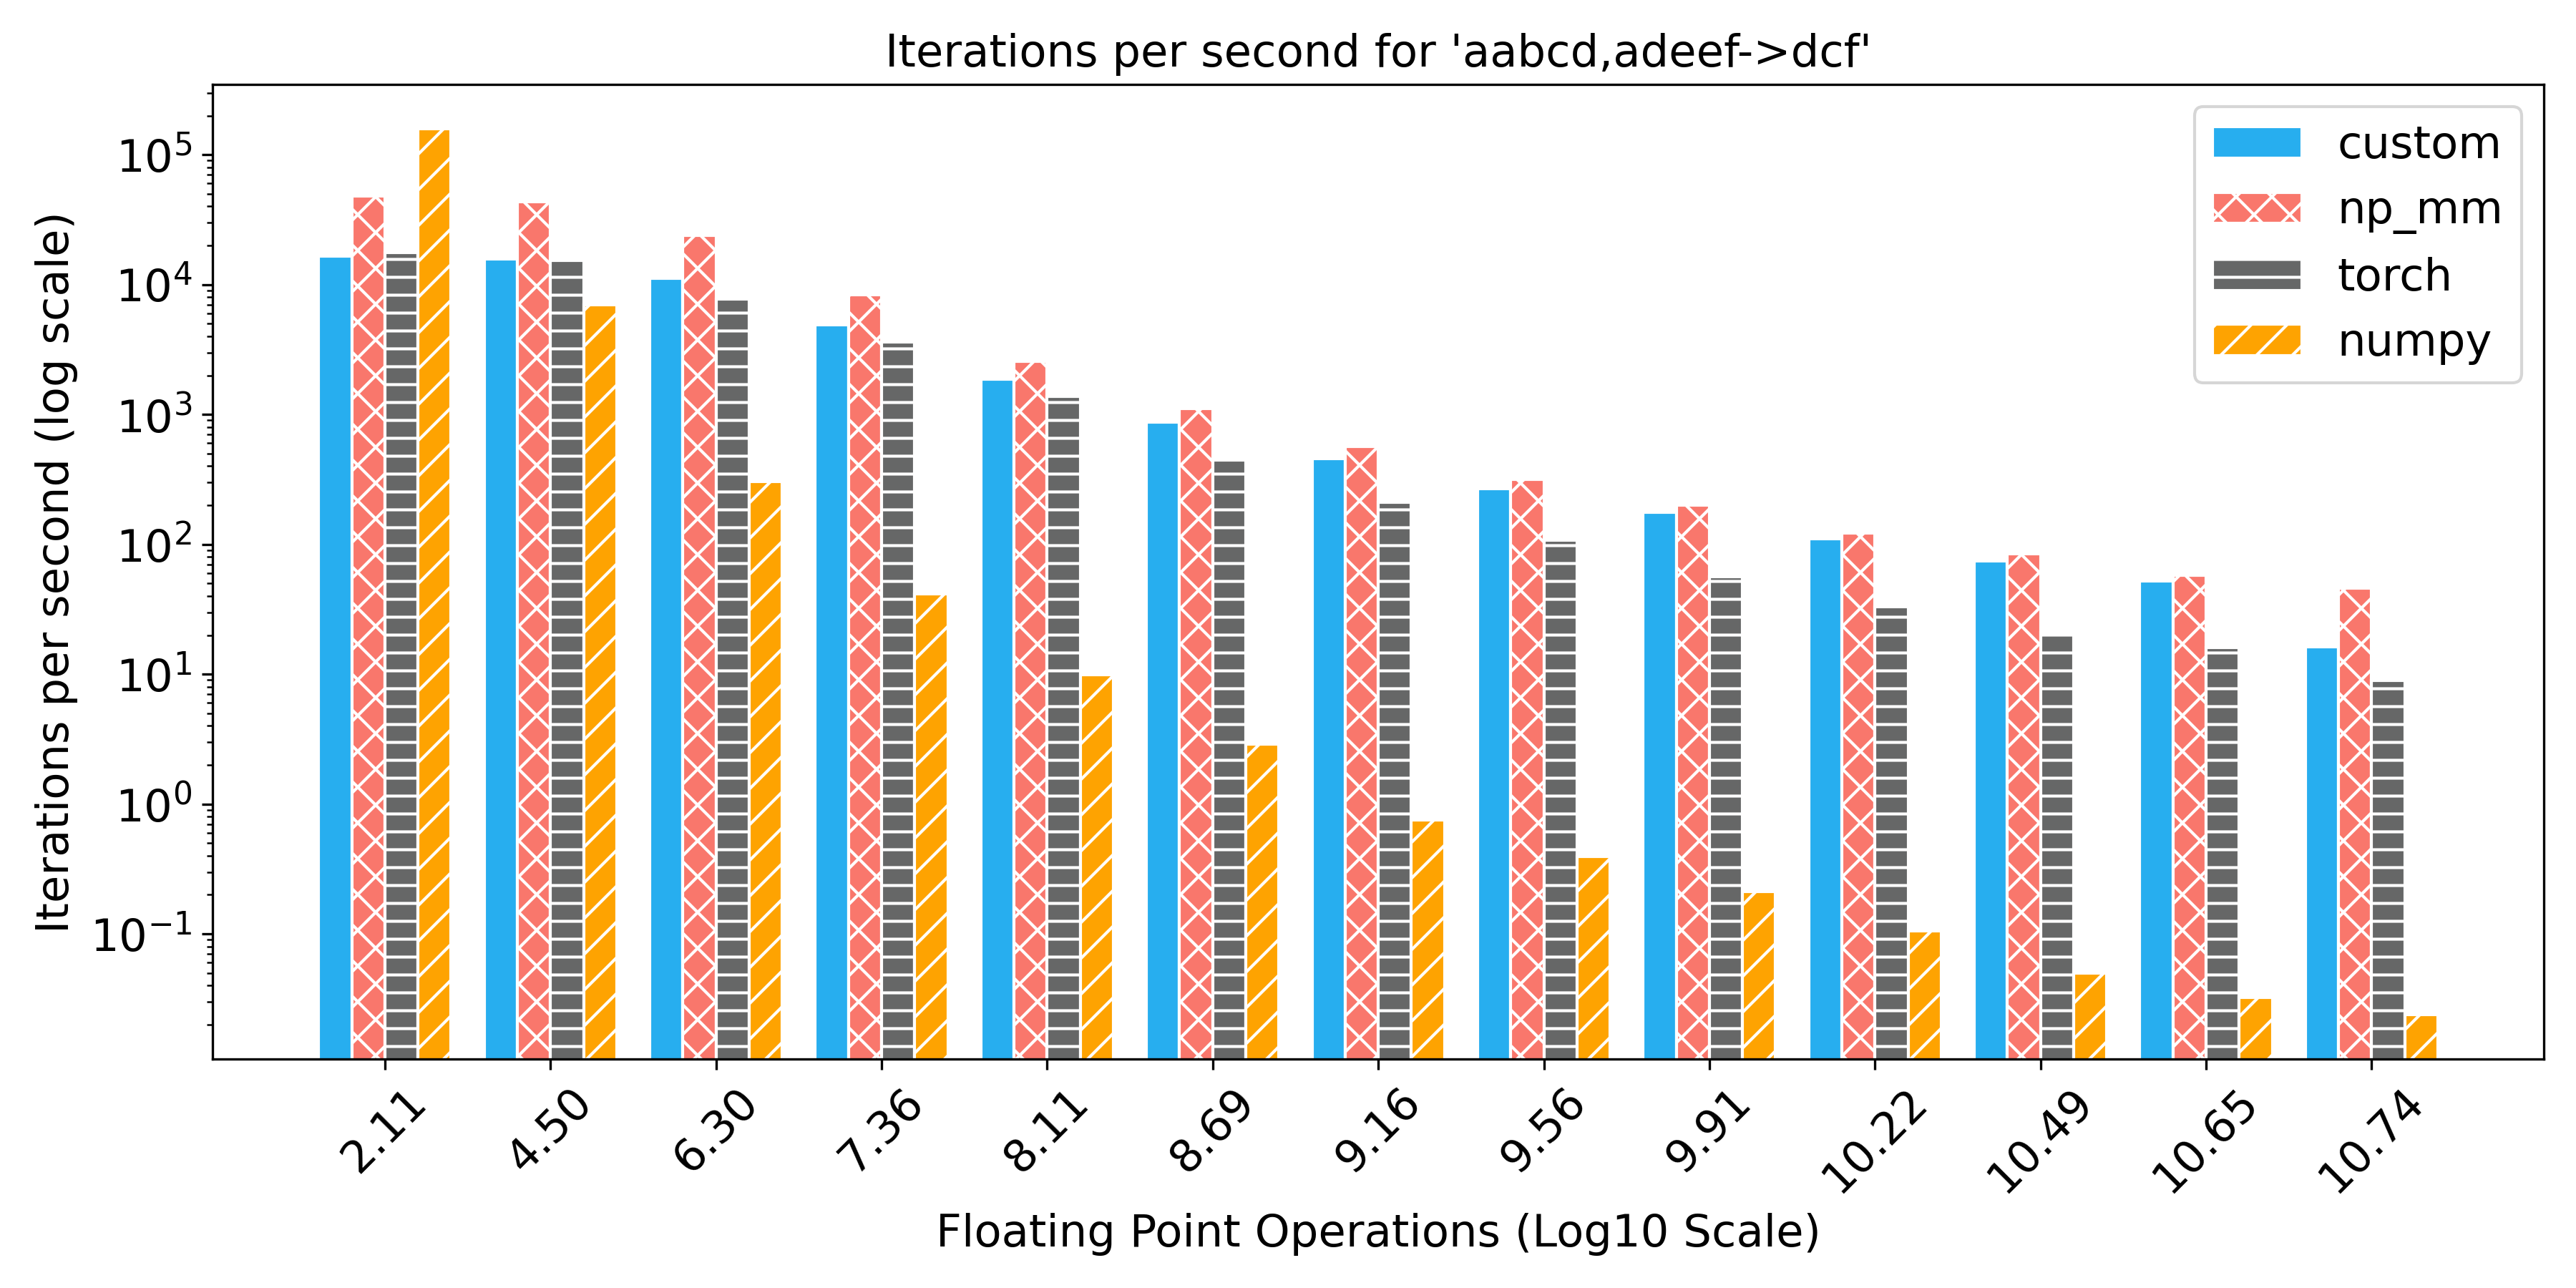
\includegraphics[width=1\textwidth]{images/aabcd_adeef__dcf.png}  % Include your image
    \caption{Performance Comparison for the pairwise contraction with batch dimensions, traces and arbitrary indices. The x-axis depicts the number of floating point operations corresponding to the gradually increased dimension sizes.}
\end{figure}

\noindent While the performance of all implementations decreases for all four problems with a growing number of floating-point operations, the rate of this degration varies. Numpy performs better than all the other backends for low counts of floating-point operations in all four contractions, as depicted in Figure~\ref{pic:all} in the appendix. However, its performance declines fastly with increasing problem size. For the largest problems, our algorithm with the np\_mm backend emerges as the most efficient method across all cases, as can be seen in Table~\ref{tab:flop_comp}.

\begin{table}[H]
    \caption{Performance comparison for the largest tensor contractions of the respective problems across the different engines, scaled to the best performance.}
    \label{tab:flop_comp}
    \centering
    {\scriptsize  % Apply the scriptsize font to the entire table
    \begin{tabularx}{\textwidth}{>
    {\raggedright\arraybackslash}p{4cm} >
    {\centering\arraybackslash}X >
    {\centering\arraybackslash}X >
    {\centering\arraybackslash}X >
    {\centering\arraybackslash}X >
    {\centering\arraybackslash}X}
        \toprule
        \textbf{\scriptsize Tensor Expression} & \textbf{\scriptsize FLOPS}& \textbf{\scriptsize Custom} & \textbf{\scriptsize np\_mm} & \textbf{\scriptsize Numpy} & \textbf{\scriptsize Torch} \\
        \midrule
        $aabcd,adeef\rightarrow dcf$ &10.74& 0.35 &\textbf{ 1} & 0.00043 & 0.19 \\
        $abcd,adef\rightarrow dbef$ &10.93& 0.36 &\textbf{ 1} & 0.0014  & 0.72 \\
        $aabcd,adeef\rightarrow bcf$ &10.74& 0.15 &\textbf{ 1} & 0.001   & 0.42 \\
        $abcd,adef\rightarrow cbef$ &10.93& 0.11 &\textbf{ 1} & 0.03    & 0.98 \\
        \bottomrule
    \end{tabularx}
    }
\end{table}


\section{Einsum Benchmark} 
We ran the 28 problems from the einsum\_benchmark dataset~\cite{blacher2024einsum} that are small enough to fit on our machine and have a non-complex data type. An overview over the properties of the einsum expressions can be found in the appendix in Table~\ref{tab:all_properties} and the performance results in Table~\ref{tab:all_performance}.
 For our performance discussion we chose five representative problems that depict the differences between the four einsum engines. Table \ref{tab:properties} lists the relevant properties of these problems.
\begin{table}[H]
    \caption{Instance data with instance name, number of tensors and the size of the biggest intermediate tensor.}
    \label{tab:properties}
    \centering
    {\tiny  % Apply the scriptsize font to the entire table
    \begin{tabularx}{\textwidth}{>
    {\raggedright\arraybackslash}p{4cm} >
    {\centering\arraybackslash}X >
    {\centering\arraybackslash}X >
    {\centering\arraybackslash}X}
        \toprule
        \textbf{\tiny Instance Name} & \textbf{\tiny Number of Tensors} & \textbf{\tiny Biggest Intermediate Tensor} & \textbf{\tiny Data Type} \\
        \midrule
        wmc\_2023\_152 & 40489 & 16384 & float64 \\
        mc\_2023\_002  & 26556 & 131072& float64 \\
        mc\_2020\_arjun\_057 & 905 & 8388608 & int32\\
        mc\_2020\_017  & 78784 & 4194304 & int32\\
        lm\_batch\_likelihood\_sentence\_4\_12d & 84 & 39398400 & float64\\
        \bottomrule
    \end{tabularx}
    }
\end{table}

\sloppy
\noindent As can be seen in Figure \ref{e_b}, Numpy performs best for problems with small intermediate tensor sizes. Our custom algorithm is more efficient for problems with data type int\_32, while PyTorch and np\_mm are most efficient for problems with the data type double.
\begin{figure}[H]
    \centering
    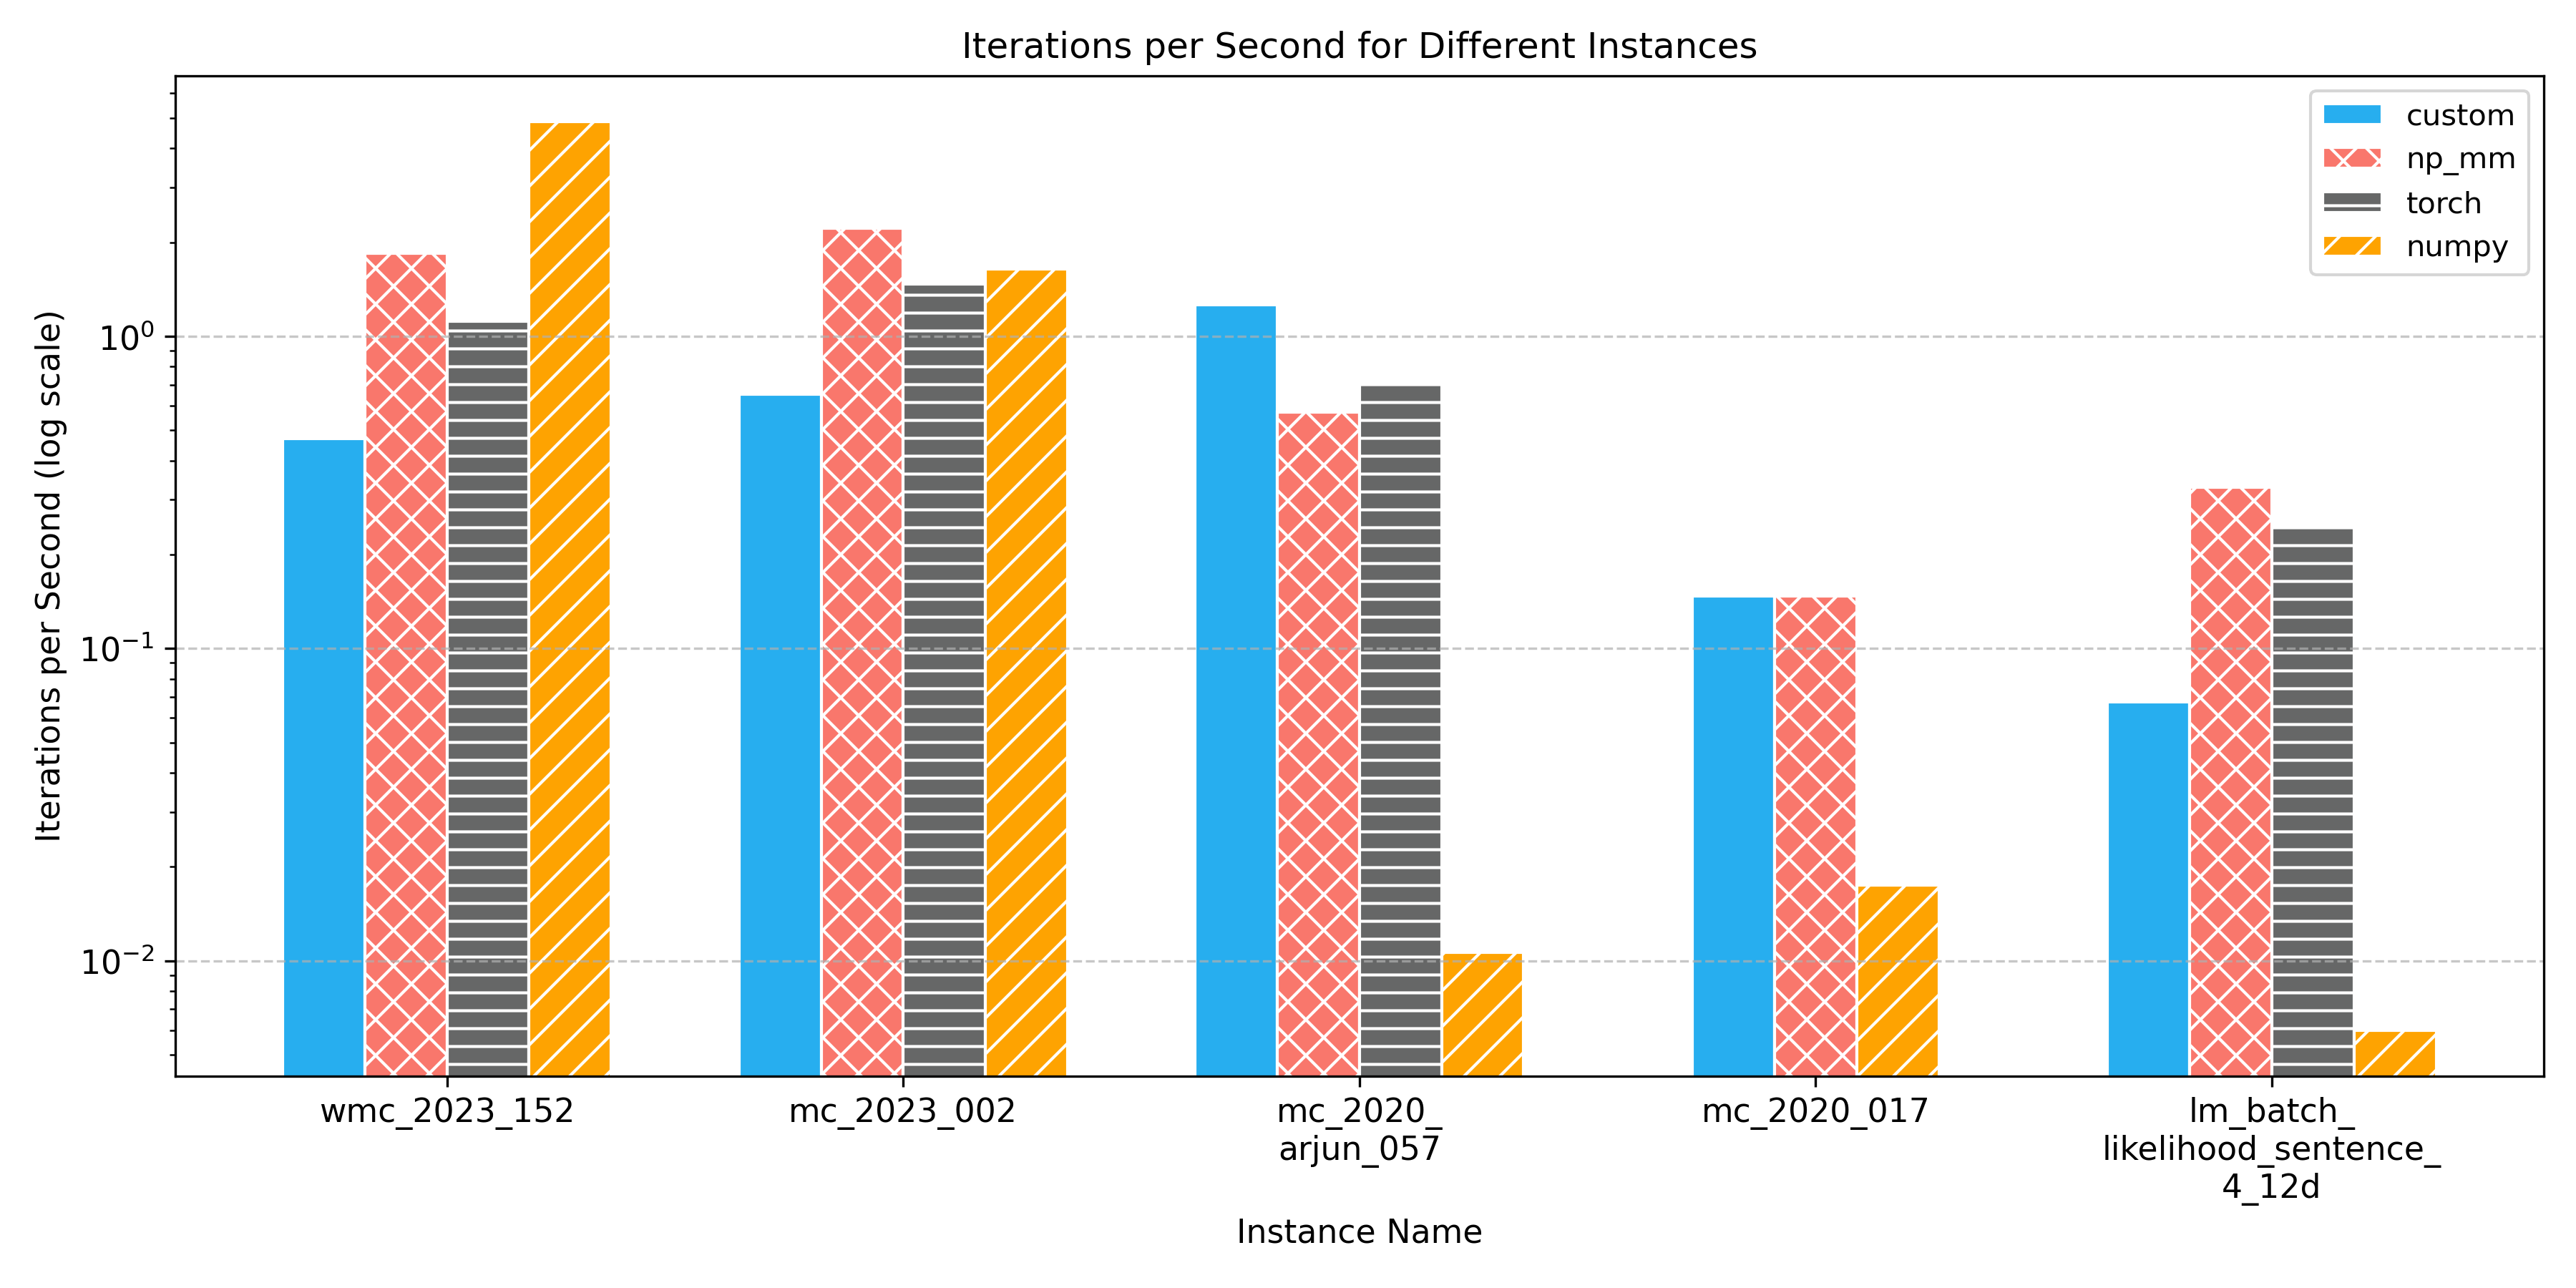
\includegraphics[width=1\textwidth]{images/einsum_five.png} 
    \caption{Performance Comparison for different problems from einsum\_benchmark~\cite{blacher2024einsum}. PyTorch was unable to compute mc\_2020\_017 due to hidden conversions from int32 to int64 during pairwise contractions.}
    \label{e_b}
\end{figure}

\noindent To further evaluate the effiency of PyTorch and np\_mm on problems with datatype double, we casted the two problems mc\_2020\_017 and mc\_2020\_arjun\_057 with datatype int\_32 to float\_64 and ran the computation again. As shown in Figure~\ref{pic:double} in the appendix, PyTorch and np\_mm both outperform the custom algorithm in this scenario.

\section{Impact of Parallelization}

\noindent To assess the impact of parallelization, we evaluated the multi-tensor contraction mc\_2020\_arjun\_046 from einsum\_benchmark~\cite{blacher2024einsum} using our custom implementation, our implementation with the np\_mm backend, and PyTorch on one and two threads. The properties of this problem can be seen in Figure~\ref{tab:arjun46_properties}. 

\begin{table}[H]
    \caption{Instance data of mc\_2020\_arjun\_046 with number of tensors and the size of the biggest intermediate tensor.}
    \label{tab:arjun46_properties}
    \centering
    {\scriptsize  % Apply the scriptsize font to the entire table
    \begin{tabularx}{\textwidth}{>
    {\raggedright\arraybackslash}p{4cm} >
    {\centering\arraybackslash}X >
    {\centering\arraybackslash}X >
    {\centering\arraybackslash}X}
        \toprule
        \textbf{\scriptsize Instance Name} & \textbf{\scriptsize Number of Tensors} & \textbf{\scriptsize Biggest Intermediate Tensor} & \textbf{\scriptsize Data Type} \\
        \midrule
        mc\_2020\_arjun\_046 & 1045 & 8388608 & int64 \\
        \bottomrule
    \end{tabularx}
    }
\end{table}
\noindent While NumPy’s batch matrix multiplication is not parallelized, our custom multi-tensor contraction shows an approximate 25\% performance improvement when increasing the thread count from one to two. PyTorch’s performance similarly improves by around 20\%. Additionally, we measured the isolated performance of our custom BMM computation. Here, the parallelization leads to an almost 50\% speed-up when scaling from one to two threads. 

\begin{figure}[H]
    \label{threads}
    \centering
    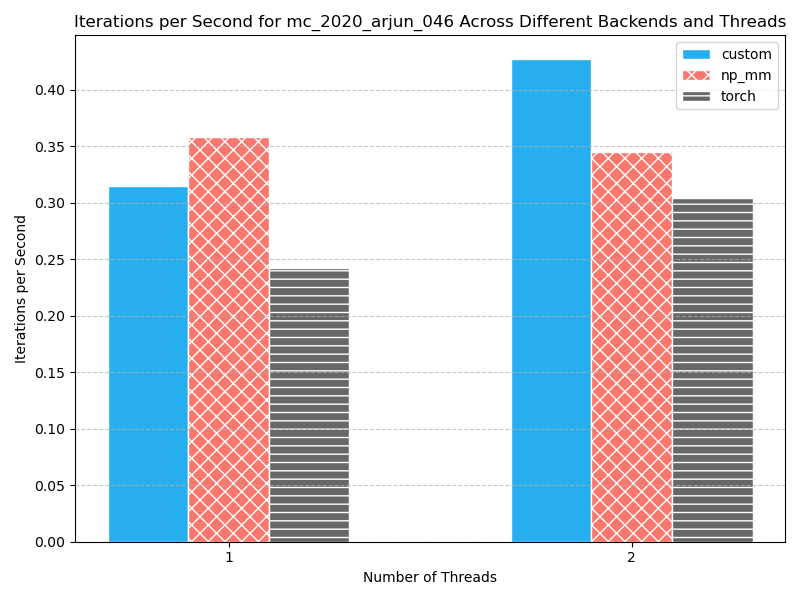
\includegraphics[width=0.6\textwidth]{images/threads.png}  % Include your image
    \caption{Iterations per second vs thread number for mc\_2020\_arjun\_046~\cite{blacher2024einsum}.}
\end{figure}
%
\chapter{Discussion}
\label{discussion}
In this chapter we seek explain the results of the experiments and discuss possible improvements to enhance our implementations efficiency.\\

\section{Result Explanation}
As described by \textcite{springer}, one of the TTBT-approaches drawbacks is the overhead induced by transposing and reshaping the tensors during pre- and post-processing. This overhead comes in costly, if the calculation is bandwith-bound which is the case for tensor contractions with relatively small tensors. This is reflected in our experiments as Numpy always outperforms Pytorch and our own implementations when the intermediate tensor size is small.\\
However, with a rising number of floating-point operations Numpy's efficiency decreases rapidely while the other implementations performance remains more stable. 
This is due to the increasing size and complexity of the tensors - while Numpy's looping approach results in poor memory access patterns, the TTBT approach used by Pytorch and our implementations ensures a more optimal cache usage.\\

\noindent Naturally, our algorithm with our custom BMM implementation is less efficient than the np\_mm version and Pytorch's engine in most cases. Even though our BMM is pararellized and blocked, it is unlikely to compete with the highly optimized linear algebra libraries that the others use for their matrix multiplications. However, our implementation performed better for some problems with data type int. A possible reason is that these libraries are optimized for floating-point arithmetics, whereas operations on integer types are handled by more generic, less-optimized code paths.\\

\section{Improvements}
Our implementation uses Numpy's einsum engine to remove traces and arbitrary indices. If the tensors are complex this can lead again to suboptimal memory access patterns. This could be avoided with a more cache oriented implementation of this operation.\\
Furthermore, we could improve our BMM by dynamically adjusting the block sizes based on the data type and cache size, and by enabling better vectorization through analyzing the data layout carefully and refactoring loop structures.

\section{Interesting stuff}
Compare it in combination with cgreedy to opt\_einsum and see, if we are better?

%
\chapter{Conclusion}
We have successfully implemented the TTBT approach for tensor contractions expressed in Einstein summation notation by mapping the preprocessed tensors to a relatively simple batch matrix multiplication. We have compared our engine with Numpy's \cite{Numpy} and PyTorch's \cite{PyTorch} einsum library on generated and real-world problems and found that our implementation can compete with these well-known libraries. Moreover, our implementation can handle a wider range of input strings than PyTorch and is more efficient for certain data types. In doing so, we proved it possible to write a simple but yet powerful engine for efficient pairwise tensor contractions that can easily be used for multi-tensor contractions given a contraction path. This engine could be further improved by enhancing memory access patterns of the preprocessing and the BMM implementation.

%
\printbibliography
%
% Change the numbering for Figures and Tables in the Appendix
\setcounter{figure}{0}
\setcounter{table}{0}
\renewcommand{\thefigure}{A.\arabic{figure}}
\renewcommand{\thetable}{A.\arabic{table}}
\chapter*{Appendix}  % No number for the chapter, use \chapter for numbering
\begin{table}[h]
    \centering
    {\scriptsize
    \caption{Number of floating-point operations for different dimension sizes for $a,b,c,d,e,f$. For the other three contractions abcd,adef$\rightarrow$dbef, aabcd,adeef$\rightarrow$bcf and abcd,adef$\rightarrow$cbef, the sizes of the tensors are changed in an analogous manner.}
    \label{tab:dimensions}
    \begin{tabular}{ccc}  
        \toprule
        \textbf{Dimension Size} & \textbf{aabcd,adeef}$\rightarrow$\textbf{dcf} & \textbf{FLOPs} \\
        \midrule
        2  & A:(2,2,2,2,2), B:(2,2,2,2,2) & 2.11  \\
        5  & A:(5,5,5,5,5), B:(5,5,5,5,5) & 4.49  \\
        10 & A:(10,10,10,10,10), B:(10,10,10,10,10) & 6.30  \\
        15 & A:(15,15,15,15,15), B:(15,15,15,15,15) & 7.36  \\
        20 & A:(20,20,20,20,20), B:(20,20,20,20,20) & 8.11  \\
        25 & A:(25,25,25,25,25), B:(25,25,25,25,25) & 8.69  \\
        30 & A:(30,30,30,30,30), B:(30,30,30,30,30) & 9.16  \\
        35 & A:(35,35,35,35,35), B:(35,35,35,35,35) & 9.56  \\
        40 & A:(40,40,40,40,40), B:(40,40,40,40,40) & 9.91  \\
        45 & A:(45,45,45,45,45), B:(45,45,45,45,45) & 10.22 \\
        50 & A:(50,50,50,50,50), B:(50,50,50,50,50) & 10.49 \\
        53 & A:(53,53,53,53,53), B:(53,53,53,53,53) & 10.65 \\
        55 & A:(55,55,55,55,55), B:(55,55,55,55,55) & 10.74 \\
        57 & A:(57,57,57,57,57), B:(57,57,57,57,57) & 10.84 \\
        59 & A:(59,59,59,59,59), B:(59,59,59,59,59) & 10.93 \\
        \bottomrule
    \end{tabular}}
\end{table}


\begin{figure}[h]
    \label{pic:all}
    \centering
    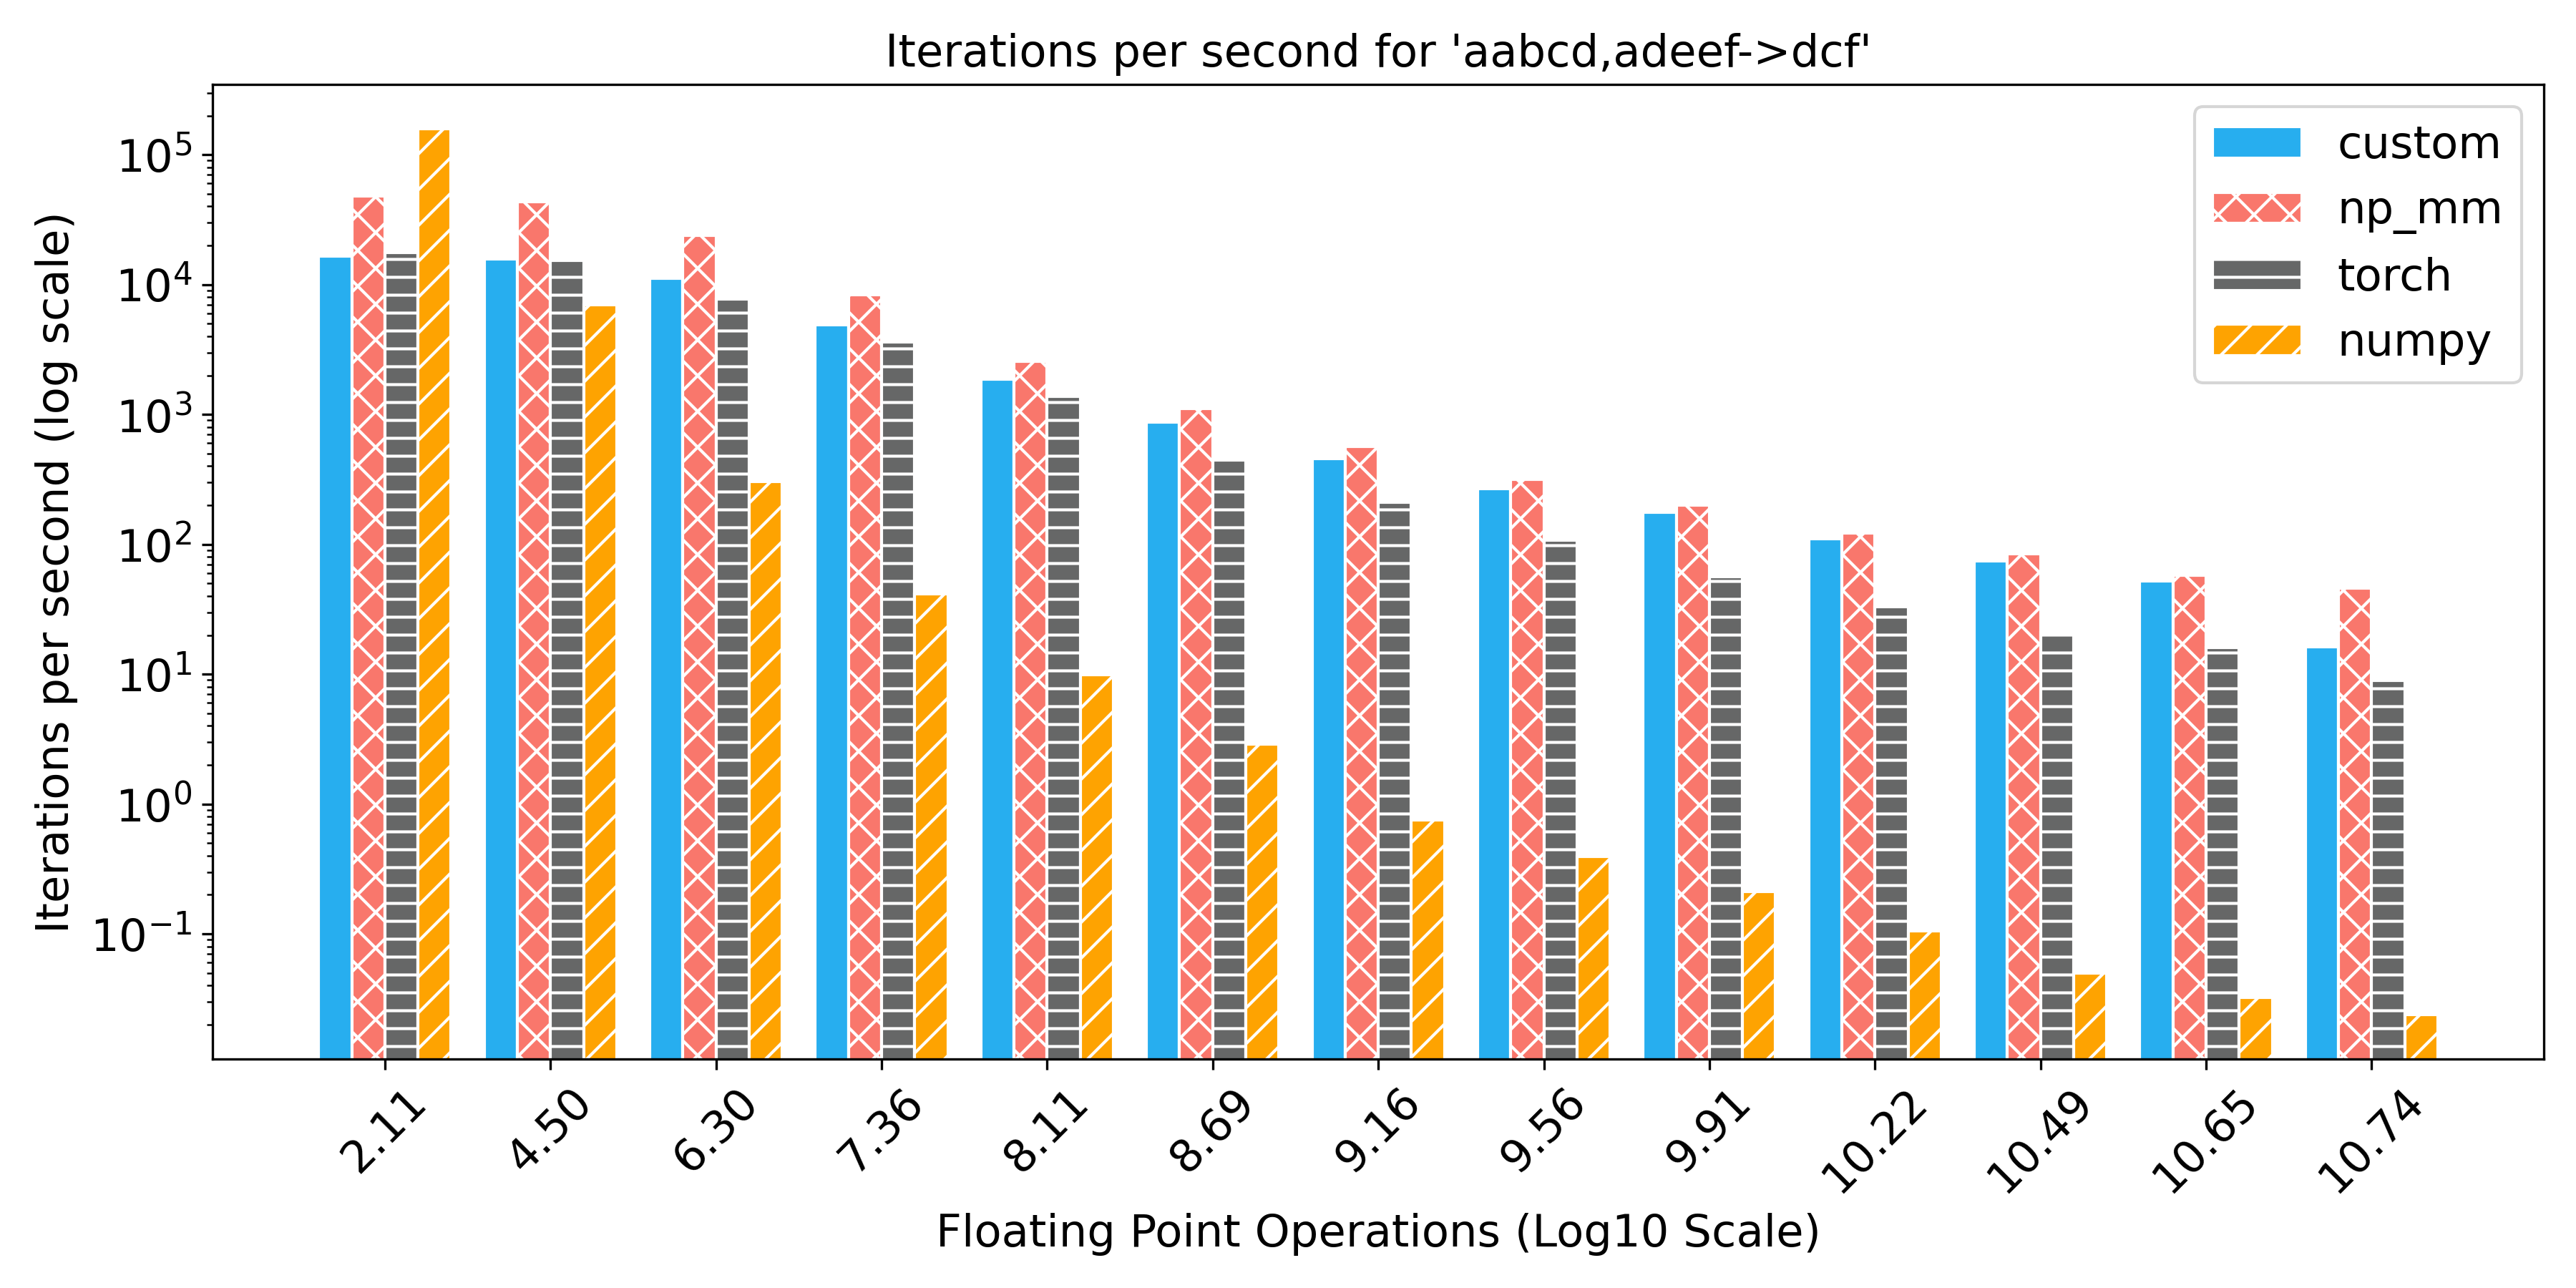
\includegraphics[width=0.49\textwidth]{images/aabcd_adeef__dcf.png} 
    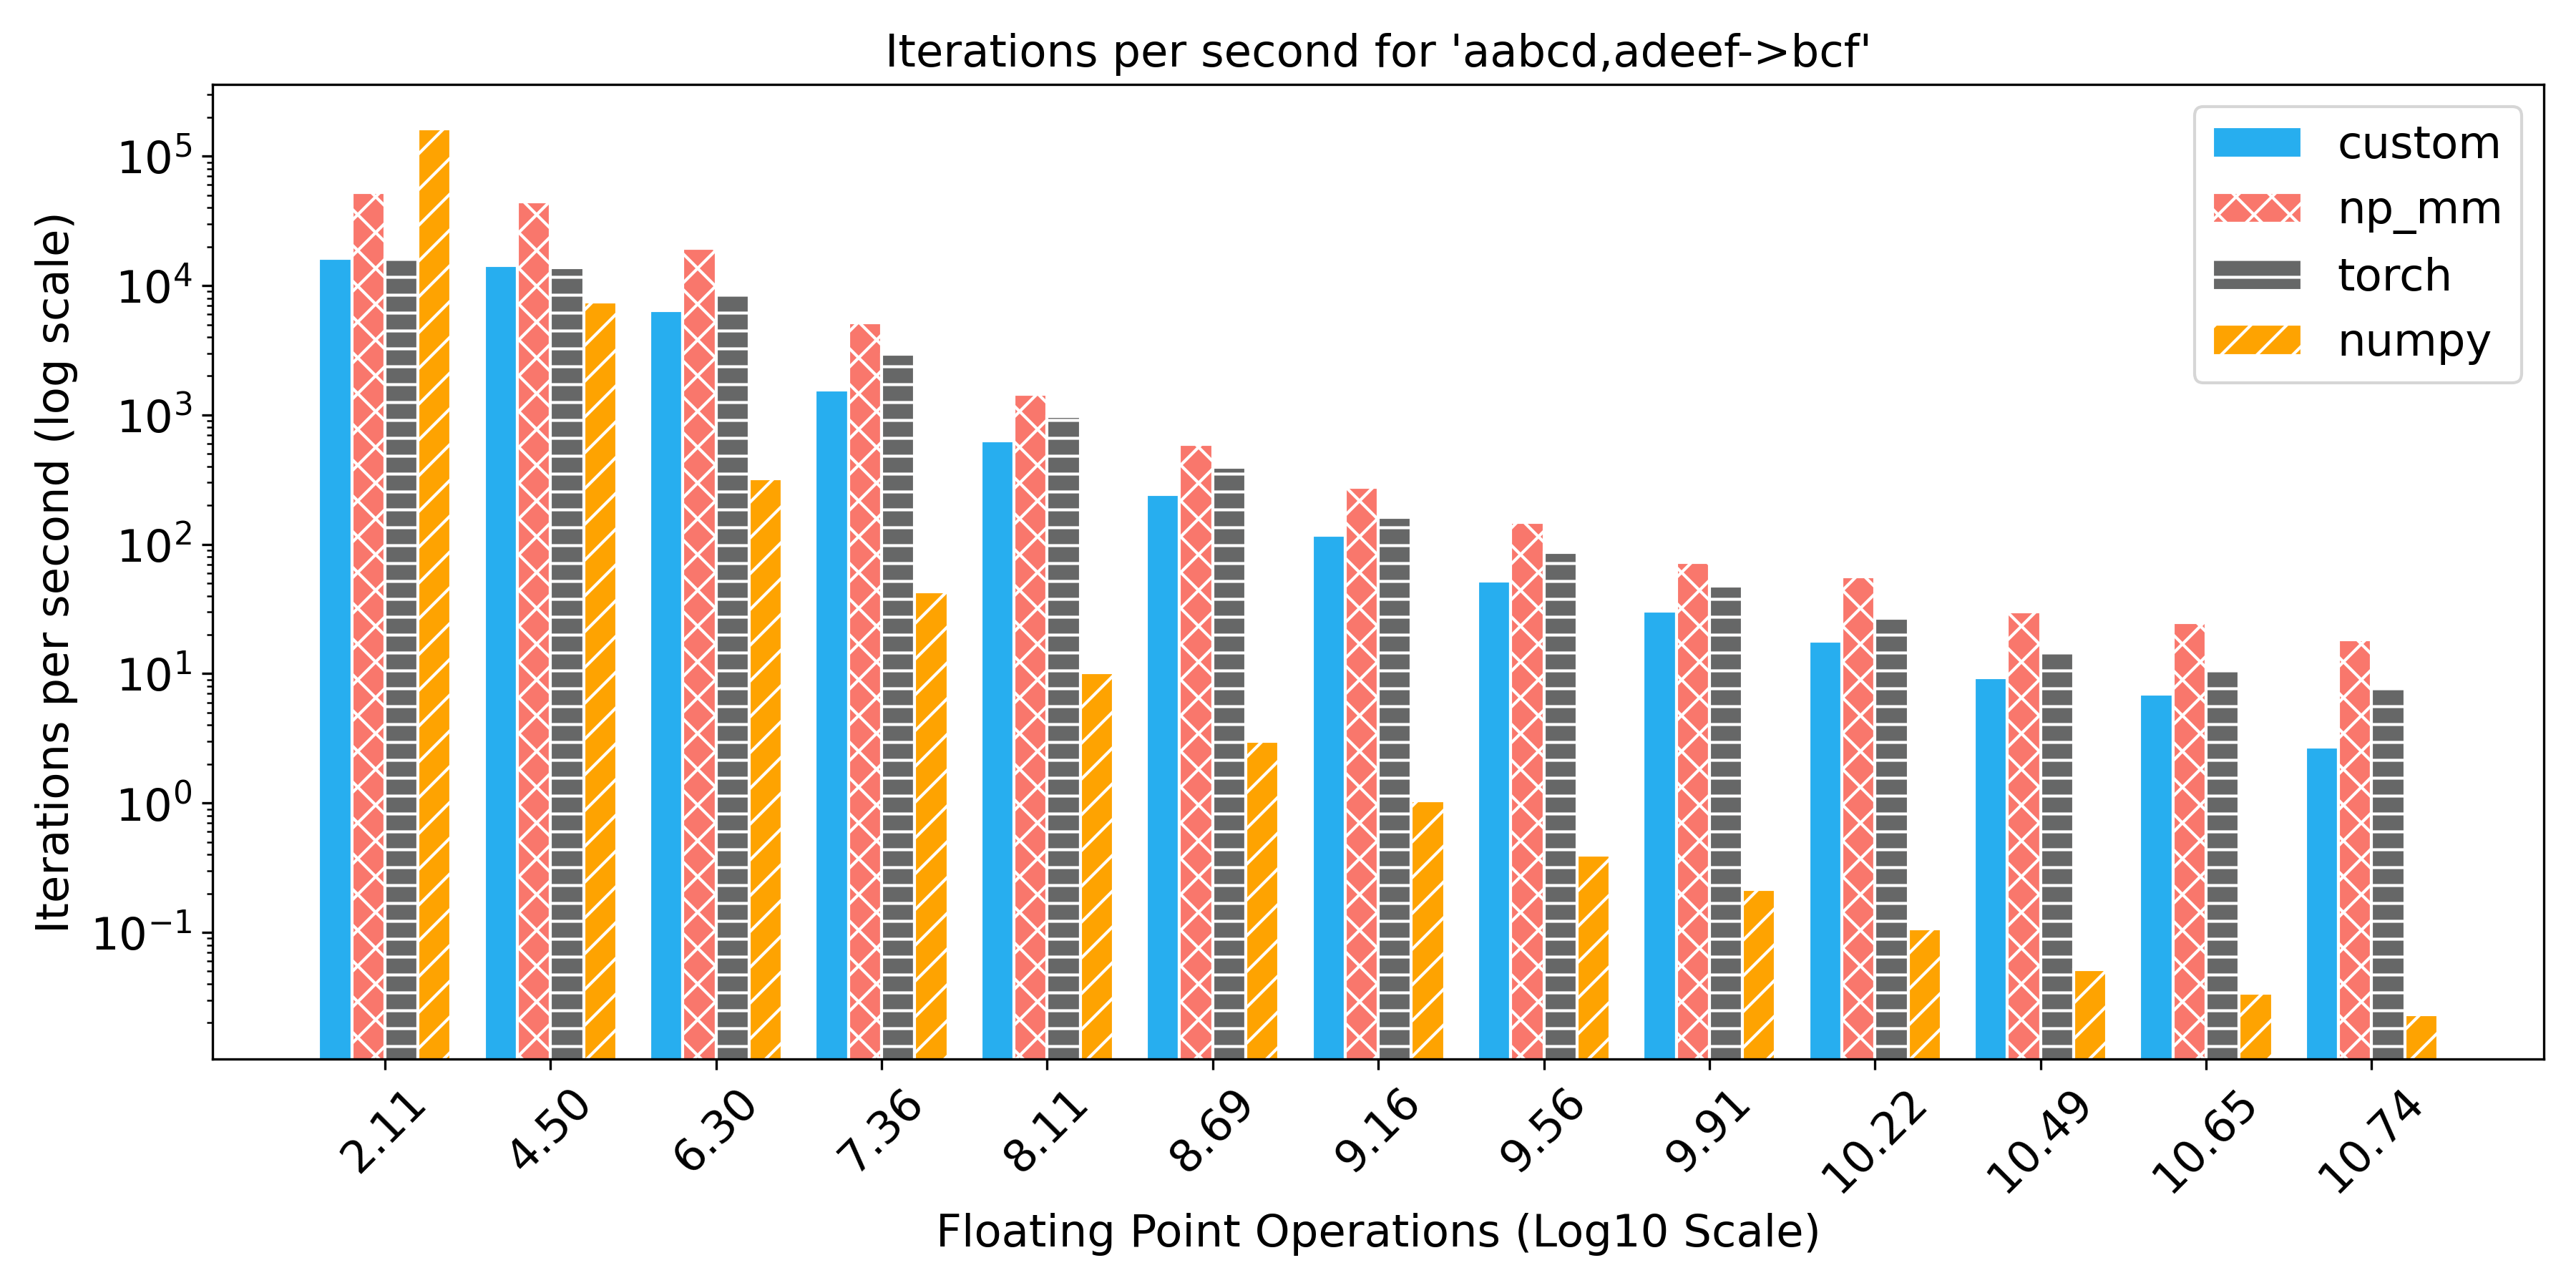
\includegraphics[width=0.49\textwidth]{images/aabcd_adeef__bcf.png} \\
    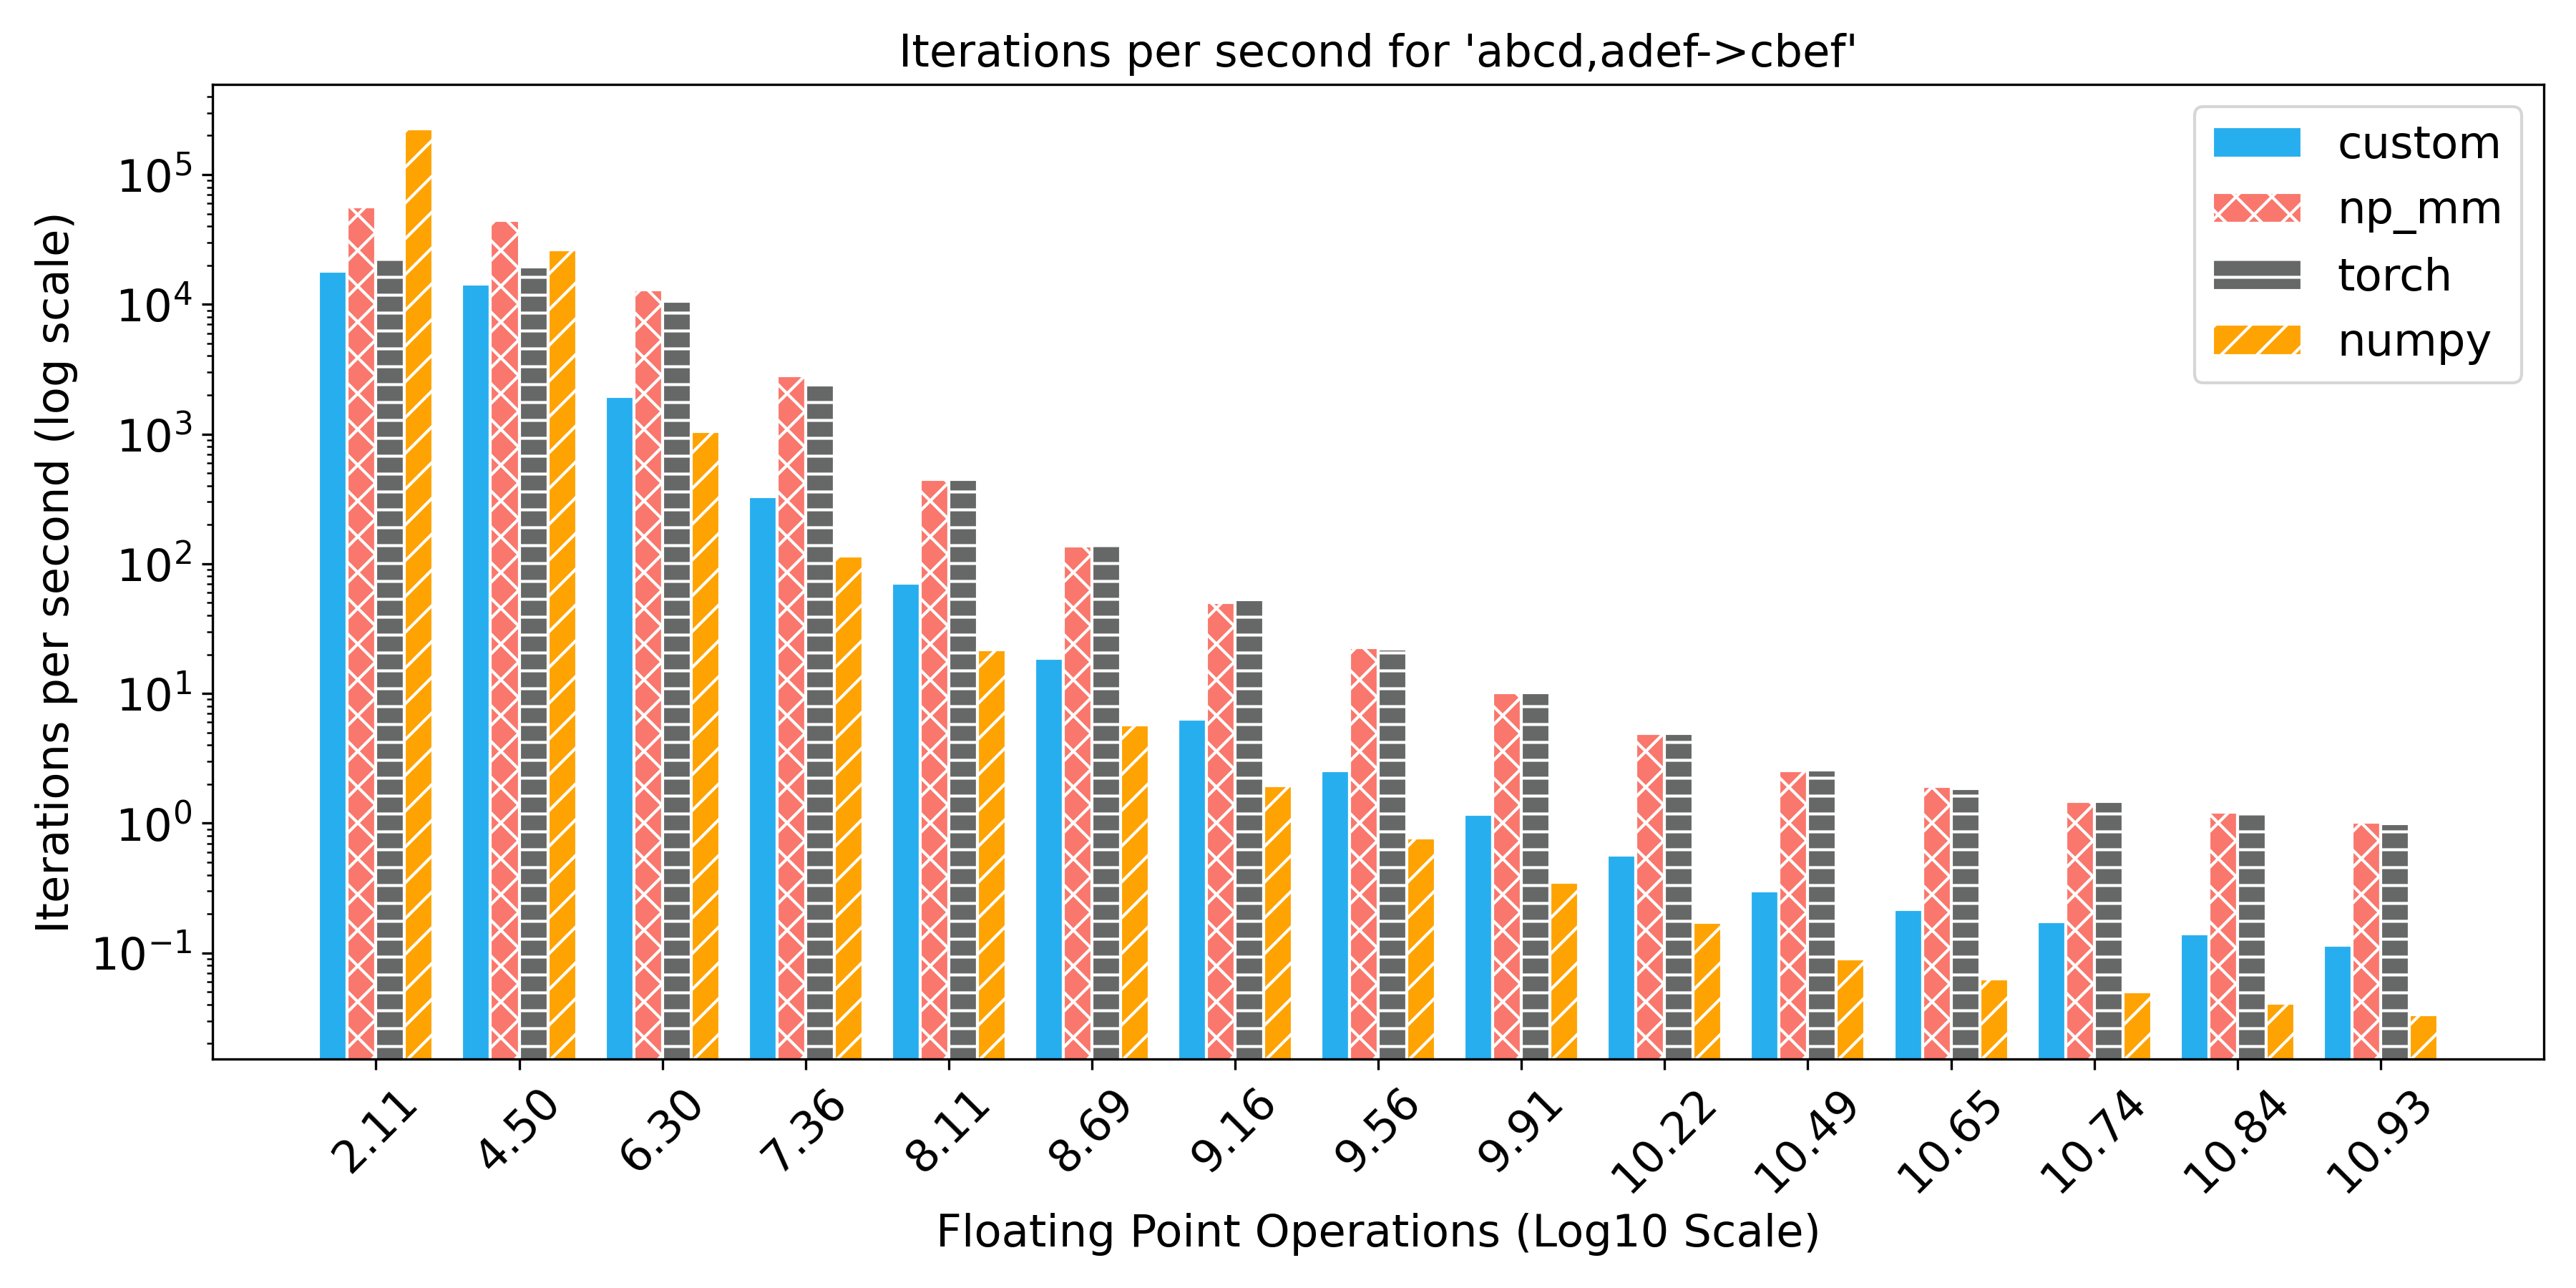
\includegraphics[width=0.49\textwidth]{images/abcd_adef__cbef.png}
    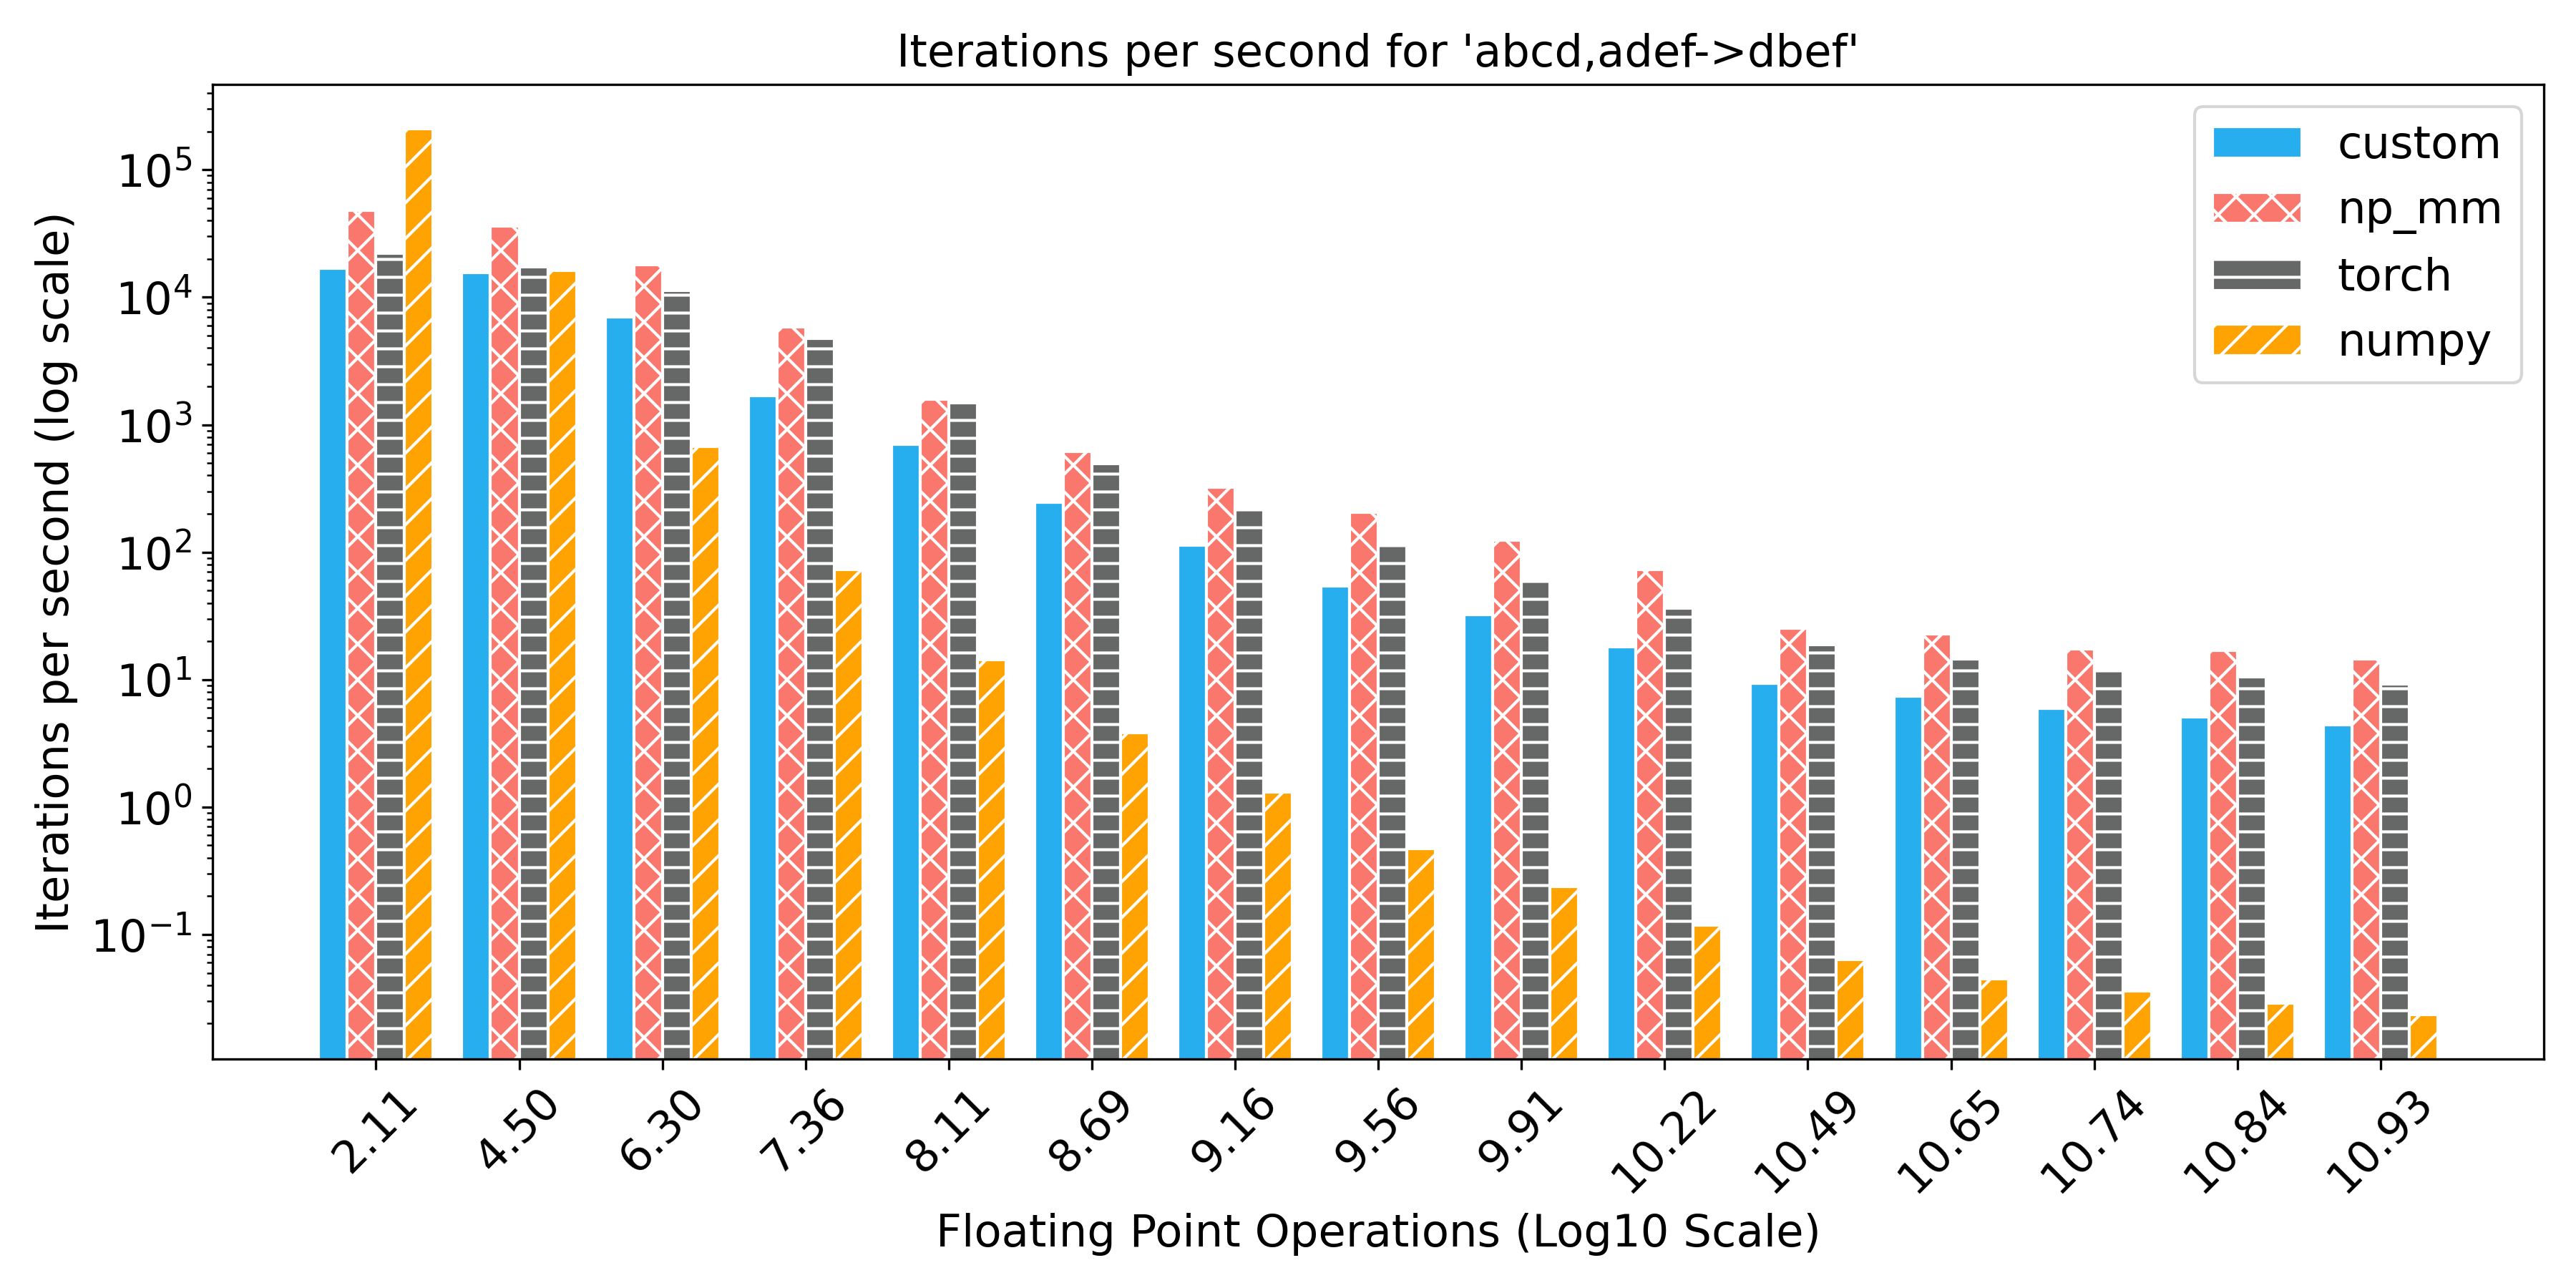
\includegraphics[width=0.49\textwidth]{images/abcd_adef__dbef.png}
    % Include your image
    \caption{Performance of the four backends over all four pairwise contractions. In all plots, the x-axis depicts the number of floating point operations corresponding to the gradually increased dimension sizes. }
\end{figure}


%\includepdf[pages=-]{chapters/Eigenständigkeitserklärung.pdf}

\end{document}
